\documentclass[12pt]{report}

\usepackage[utf8]{inputenc}



\usepackage[a4paper, 12pt,  total={6in, 8in}]{geometry}



\usepackage{ragged2e} %--For text alignment

\newenvironment{frontmatter}{}{\maketitle}

\usepackage{longtable}

\usepackage{graphicx}
\usepackage{rotating}
\usepackage{amssymb,amsmath}
%% The lineno packages adds line numbers. Start line numbering with
%% \begin{linenumbers}, end it with \end{linenumbers}. Or switch it on
%% for the whole article with \linenumbers after \end{frontmatter}.
%\usepackage{lineno}
\newtheorem{theorem}{Definition}
\usepackage{subfigure}
\usepackage{lscape}
%\usepackage{datetime}

%\usepackage{fancyhdr}
% 
%\pagestyle{fancy}
%\fancyhf{}
%\rhead{Put your tit}
%\lhead{Title}
%\rfoot{Page \thepage}


\begin{document}

\begin{titlepage}
    \begin{center}
        \vspace*{0.01cm}
        \Huge
        \textbf{Report Title}
        
        \vspace{0.5cm}
        \LARGE
        Thesis Subtitle (if any)
        
        \vspace{1.5cm}
        
        Submitted by\\
        \textbf{Author Name}
         
         University Roll No.105XXXXXXXX          
        
        \vfill
        
        A project report  submitted in partial fulfillment for the degree of
       Bachelor of Technology in Computer Science \& Engineering
        
        \vspace{0.8cm}
        
        
\includegraphics[width=0.4\textwidth]{buie_logo.jpg}
        
        Department Computer Science \& Engineering\\
        Bankura Unnayani Institute of Engineering\\
        Bankura - 722 146, West Bengal, India\\
       
       {MAY}{\hspace*{0.5cm}}{2016}
       %\date{\displaydate{date}}
        
    \end{center}
\end{titlepage}
\newpage

\pagenumbering{gobble} 

\begin{center}
\vspace*{8.5cm}
\LARGE
\textit{Dedicated to my parents}

\end{center}



\newpage
{\it ``We are what our thoughts have made us; so take care about what you think. Words are secondary. Thoughts live; they travel far.''}
\begin{flushright}
- Swami Vivekananda
\end{flushright}


{\it ``Take up one idea. Make that one idea your life - think of it, dream of it, live on that idea. Let the brain, muscles, nerves, every part of your body, be full of that idea, and just leave every other idea alone. This is the way to success.''\\}

\begin{flushright}
- Swami Vivekananda
\end{flushright}

{\it ``When an idea exclusively occupies the mind, it is transformed into an actual physical or mental state.''}
\begin{flushright}
- Swami Vivekananda
\end{flushright}

{\it ``You have to dream before your dreams can come true.''}
\begin{flushright}
-Dr. A. P. J. Abdul Kalam
\end{flushright}


{\it ``Dream is not that which you see while sleeping it is something that does not let you sleep.''}
\begin{flushright}
-Dr. A. P. J. Abdul Kalam
\end{flushright}

\newpage


 \begin{center}
        \vspace*{1cm}
         \LARGE
        \textbf{Certificate of Approval}
        
        \vspace{1.5cm}
 \justify      
		The forgoing project report is hereby approved as a creditable study of Technological subject carried out and presented in a manner satisfactory to warrant its acceptance as a prerequisite with degree for which it has been submitted. It is to be understood that by this approval, the undersigned do not necessarily endorse or approve any statement made, opinion expressed or conclusion drawn there in but approve the thesis only for the purpose for which it has been submitted.        
        
        \vspace{1.5cm}
        
        Board of Examiners
        
        \begin{itemize}
        \item 
        \item
        \item
        \item
        \end{itemize}
        
        \vfill
        
       
        
        
        
    \end{center}

\newpage


\begin{center}
        \vspace*{1cm}
         \LARGE
        \textbf{Declaration}
        
        \vspace{1.5cm}
 \justify      
		I hereby declare that this submission is my own work and that, to the best of my knowledge and belief, it contains no material previously published or written by another person nor material which has been accepted for the award of any other degrees or diplomas of the university or other institutes of higher learning, except which due acknowledgment has been made in this text.         
        
        \vspace{5.5cm}
        
  \begin{flushleft}
   ...............................................\\
      \hspace{2.5cm}Signature
\end{flushleft}        
      
 
        
        \vfill
        
       
        
        
        
    \end{center}



\newpage
\begin{center}
        \vspace*{1cm}
         \LARGE
        \textbf{Certificate}
        
        \vspace{1.5cm}
 \justify      
		This is certified that the work contained in this report entitled, TITLE, by NAME, has been carried out under the supervision of the undersign and this work has not been submitted elsewhere for any other degree.       
        
        \vspace{2.5cm}
 \small       
  \begin{flushleft}
(Signature of the Supervisor)\\
Mr. X Y, Assistant Professor, Department of CSE\\
Bankura Unnayani Institute of Engineering\\
Bankura, West Bengal

\vspace{1.5cm}

(Signature of the Co-supervisor)\\
Mr. X Y, Assistant Professor, Department of CSE\\
Bankura Unnayani Institute of Engineering\\
Bankura, West Bengal

\vspace{1.5cm}

(Signature of the HoD)\\
Mr. X Y, Associate Professor, Department of CSE\\
Bankura Unnayani Institute of Engineering\\
Bankura, West Bengal


\end{flushleft}        
      
 
        
        \vfill
        
       
        
        
        
    \end{center}
\newpage

\begin{center}
        \vspace*{1cm}
         \LARGE
        \textbf{Acknowledgments}
        
        \vspace{1.5cm}
 \justify      
		I hereby wish to express my sincere gratitude and respect to Assistant Prof. X X, Dept. of CSE, Bankura Unnayani Institute Of Engineering, Bankura under whom I had proud privilege to work. His valuable guidance and encouragement have really led me to the path of completion of this project. Any amount of thanks would not be enough for the valuable guidance of my supervisor. 
I would also like to thank all the faculty member of CSE dept. for their devoted help. I also cordially thank all laboratory assistants for their cooperation.
Finally, I would like to pen down my gratitude towards my family members for their continuous support and encouragement. It would have not been possible to complete my work without their support.
   
        
     
        
        \vfill
        
       
        
        
        
    \end{center}
    


\newpage
\vspace*{1cm}
\begin{center}
\LARGE
\textbf{Abstract}
\end{center}

\justify
 your abstract begins here.........\\
 Write your abstract in maximum 200-300 words.
 
 \vspace*{1cm}
 \smallskip
\noindent \textbf{Keywords.} list of keywords.
 Put atleast 6-8 keywords of your thesis work separated by coma(,)
 

\newpage
%\addcontentsline{toc}{chapter}{*}
\tableofcontents



\listoffigures


\newpage

\listoftables

\newpage
%\setcounter{page}{1}
\pagenumbering{arabic}
\chapter{Introduction}
%\justify
This  is  the  second  paragraph. Hello, here is some text without 
a meaning.  This text should show what 
a printed text will look like at this place.  If you read this text, 
you will get no information.  Really?  Is there no information?  Is there 
a difference between this text and some nonsense like not at all!  A 
blind text like this gives you information about the selected font, how 
the letters are written and an impression of the look.  This text should
contain all letters of the alphabet and it should be written in of the
original language.There is no need for special content, but the length of
words should match the language.

\newpage

\chapter{Background Theory}

{\bf Mathematical Equations}\\

You can write your mathematical equation as like in Eq.(\ref{eq:1}).

\begin{equation}
\label{eq:1}
X_{i}^{2}+Y_{j}^{2}=Z_{k}^{2}
\end{equation}


\newpage

\chapter{Review}

\newpage
\chapter{Materials \& Methods}
\section{Example of Table}



\begin{table}[h]
\centering
\caption{Table to test captions and labels}
\label{table:1}
\begin{tabular}{ |c| c| c| }
\hline
 cell1 & cell2 & cell3 \\ 
 \hline
 cell4 & cell5 & cell6 \\ 
 \hline 
 cell7 & cell8 & cell9   \\ 
 \hline
\end{tabular}

\end{table}




The table \ref{table:2} is an example of referenced \LaTeX elements.
\begin{sidewaystable}[h]
%\begin{table}[]
\centering
\caption{Table to test captions and labels}
\label{table:2}
\begin{tabular}{ |c| c| c| }
\hline
 cell1 & cell2 & cell3 \\ 
 \hline
 cell4 & cell5 & cell6 \\ 
 \hline 
 cell7 & cell8 & cell9   \\ 
 \hline
\end{tabular}

%\end{table}
\end{sidewaystable}




{\bf Multi-page tables}\\

If you have to insert a very long table, which takes up two or more pages in your document, use the longtable package. First, add to the preamble the line

\begin{verbatim}
\usepackage{longtable}
\end{verbatim}


\begin{longtable}[c]{| c | c |}
 \caption{Long table caption.\label{long}}\\
 
 \hline
 \multicolumn{2}{| c |}{Begin of Table}\\
 \hline
 Something & something else\\
 \hline
 \endfirsthead
 
 \hline
 \multicolumn{2}{|c|}{Continuation of Table \ref{long}}\\
 \hline
 Something & something else\\
 \hline
 \endhead
 
 \hline
 \endfoot
 
 \hline
 \multicolumn{2}{| c |}{End of Table}\\
 \hline\hline
 \endlastfoot
 
 Lots of lines & like this\\
 Lots of lines & like this\\
 Lots of lines & like this\\
 Lots of lines & like this\\
 Lots of lines & like this\\
 Lots of lines & like this\\
 Lots of lines & like this\\
 Lots of lines & like this\\
 ...
 Lots of lines & like this\\
 \end{longtable}

%The table \ref{table:3} is an example of referenced \LaTeX elements in landscape.
%
%\begin{landscape}
%
%\begin{table}[bth]
%\begin{center}
%\caption{Table to test captions and labels}
%\label{table:3}
%\begin{tabular}{ |c| c| c| }
%\hline
% cell1 & cell2 & cell3 \\ 
% \hline
% cell4 & cell5 & cell6 \\ 
% \hline 
% cell7 & cell8 & cell9   \\ 
% \hline
%\end{tabular}
%
%\end{center}
%\end{table}
%
%\end{landscape}

\newpage

\chapter{Results \& Discussion}

The graph is given in Fig.~\ref{fig:logo}.

\begin{figure}[!bth]
\center
\label{fig:logo}
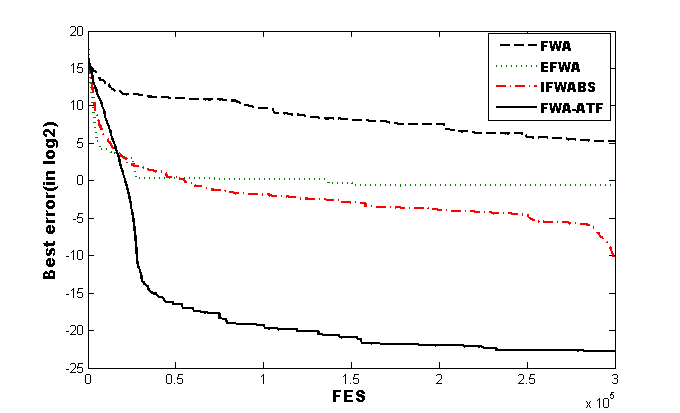
\includegraphics[scale=0.6]{f1.png}
\caption{Graph}
\end{figure}


If you need to place multiple images all together, use this...


\begin{figure}[!h]
  \centering
   \begin{tabular}{l l l}
  \subfigure[\label{db1mri1}]{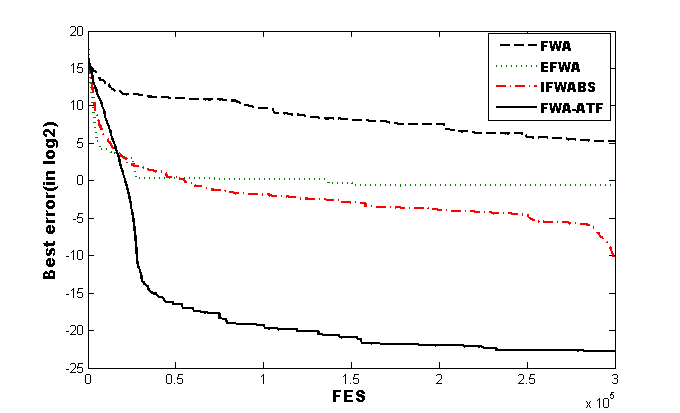
\includegraphics[width=1.4in,height=1.2in]{f1.png}}   &
   
  \subfigure[\label{db1mri2}]{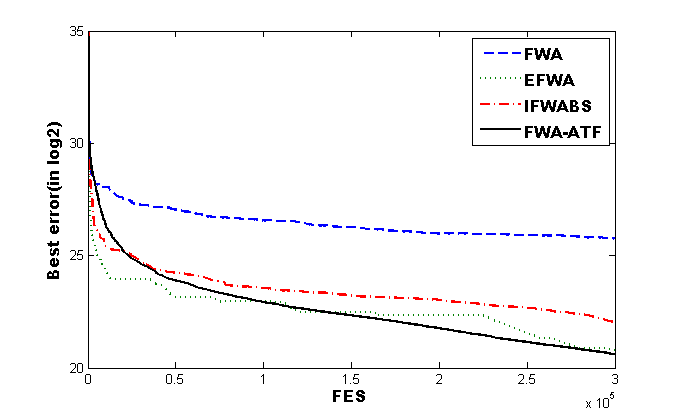
\includegraphics[width=1.4in,height=1.2in]{f2.png}}   &
 
  \subfigure[]{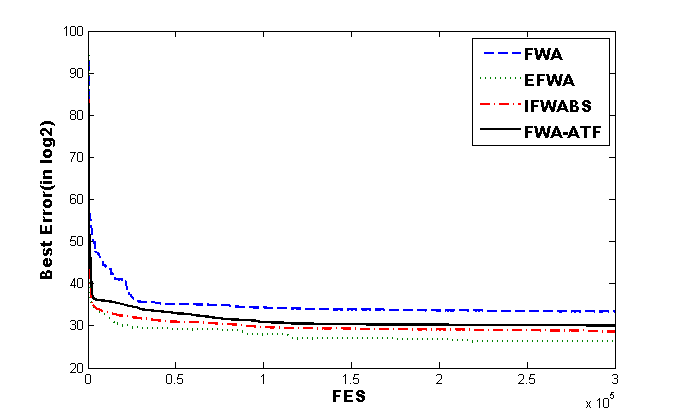
\includegraphics[width=1.4in,height=1.2in]{f3.png}}  \\

  \subfigure[]{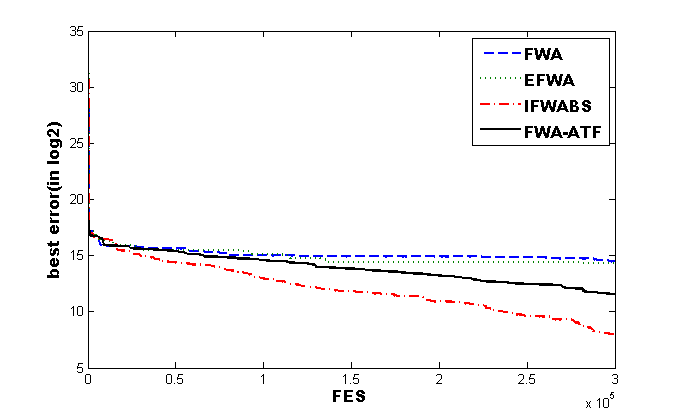
\includegraphics[width=1.4in,height=1.2in]{f4.png}}   &
 
  \subfigure[]{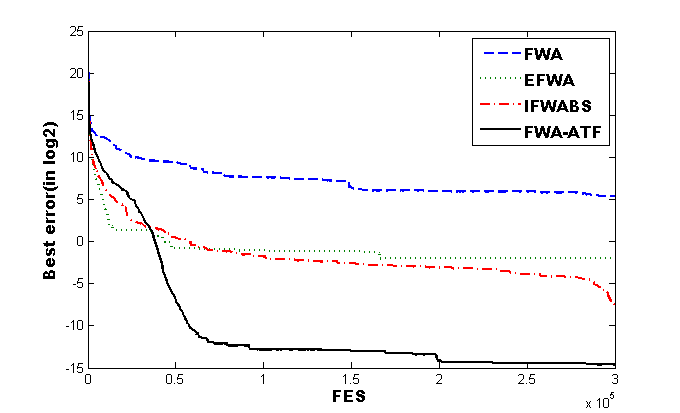
\includegraphics[width=1.4in,height=1.2in]{f5.png}}   &

  \subfigure[]{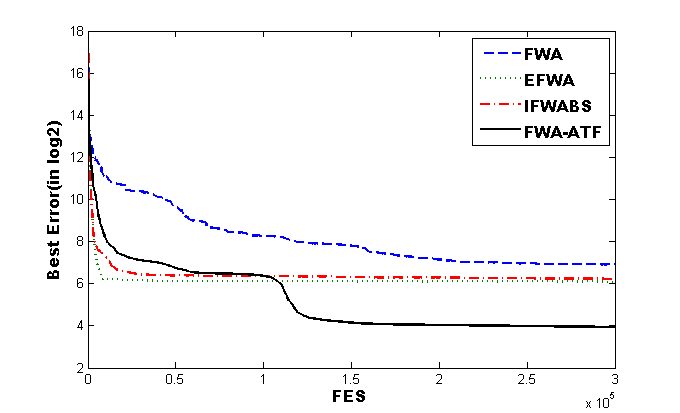
\includegraphics[width=1.4in,height=1.2in]{f6.png}}   \\
   \end{tabular}   
  \caption{put the caption}.
 \label{fig:db1}
\end{figure}



\newpage

\chapter{Conclusions}

\newpage

\chapter{Future Works}
Here you can outline the future scopes of your work..........
\newpage

\chapter*{List of Publications}
\begin{enumerate}
\item Author's name, Title, Conference, date, place, year, pp.~xx-xx.
\item Author's name, Title, Journal, Vol~X, No.~X, Year, pp.~xx-xx.
\end{enumerate}
\newpage
\begin{thebibliography}{00}
\bibitem{Derrac}
J. Derrac, S. Garcia, D. Molina and  F. Herrera, A practical tutorial on the use of nonparametric statistical tests as a methodology for comparing evolutionary and swarm intelligence algorithms. Swarm and Evolutionary Computation, 1(2011), 3-–18
\end{thebibliography}


\end{document}
